\chapter[Automated detection of Epileptic ripples]{Automated detection of Epileptic Ripples in MEG using beamformer-based Virtual Sensors}
\label{ch:5}
\textbf{Published as:} 
Migliorelli, C., Alonso J.F., Romero S., Ma\~nanas, Nowak R. and Russi A.
Automated detection of Epileptic Ripples in MEG using beamformer-based Virtual Sensors. \textit{Journal of Neural Engineering} \textit{Accepted Manuscript}

doi: 10.1088/1741-2552/aa684c

Impact Factor: 3.493; Position 10 of 76 (Q1) BIOMEDICAL ENGINEERING.



\textbf{Abstract:} \textit{Objective.} In epilepsy, high-frequency oscillations (HFOs) are considered events highly linked to the seizure onset zone (SOZ). The detection of HFOs in noninvasive signals such as scalp EEG and MEG is still a challenging task. The aim of this study was to automatize the detection of ripples in MEG signals reducing the high-frequency noise using beamformer-based virtual sensors (VS) and applying an automatic procedure exploring the time-frequency content of the detected events. \textit{Approach.} 200 seconds of MEG signals and simultaneous iEEG were selected in nine patients with refractory epilepsy. A two-stage algorithm was implemented. Firstly, beamforming was applied to the whole head to delimitate the region of interest (ROI) within a coarse grid of MEG-VS. Secondly, a beamformer using a finer grid in the ROI was computed. The automatic detection of ripples was performed using the time-frequency response provided by the Stockwell Transform. The performance was evaluated by comparing with simultaneous iEEG signals. \textit{Main results.} For the nine subjects, ROIs were located within the seizure-generating lobes. Precision and sensitivity values were 79.18\% and 68.88\%, respectively, considering iEEG detected events as benchmark. A higher number of ripples were detected inside the ROI compared to the same region in the contralateral lobe. \textit{Significance.}  The evaluation of interictal ripples using noninvasive techniques can help in the delimitation of the EZ and guide the placement of intracranial electrodes. This is the first study that automatically detects ripples in MEG in the time domain located within the clinically expected epileptic area taking into account the time-frequency characteristics of the events through the whole signal spectrum. The algorithm was tested against intracranial recordings, the current gold standard. Further studies should explore this approach to enable the localization of noninvasively recorded HFOs to help during pre-surgical planning and to reduce the need for invasive diagnostics.

\textbf{Keywords:} high frequency oscillations, epilepsy, MEG, ripples, beamformer.

\section{Introduction}

Epilepsy is a neurological disorder that affects about 1\% of the world population \citep{Ramey2013}. The most common therapeutic treatment relies on antiepileptic drugs (AEDs) which aims to reduce or eliminate seizures. Approximately 20\% to 40\% of patients diagnosed with epilepsy become refractory to treatment \citep{Liu2015c}. For these patients, the most frequent therapeutic alternative is the neurosurgical resection of the epileptogenic zone (EZ), defined as the cortex area that is necessary and sufficient for initiating the epileptic discharges and whose removal is necessary for complete abolition of seizures \citep{Schuele2008}.

In current practice, the epileptogenic zone is approximated by the seizure onset zone (SOZ), defined as the area where the clinical seizures originate. The delimitation of this area is often done by the presurgical analysis with intracranial electroencephalography (iEEG) \citep{Rosenow2001} during the pre-ictal and ictal periods. In several recent studies, high-frequency oscillations (HFOs) have been evaluated as a specific biomarker for epileptogenicity in iEEG \citep{Jacobs2012,Fujiwara2012,Sun2015}. These fast oscillations appear in the frequency range of 80-500Hz, classified into ripples (80-200Hz) and fast ripples (200-500Hz) and are defined as spontaneous patterns above the baseline, clearly distinguished from noise and with at least four oscillations \citep{Worrel2012}. They can be recorded during the interictal period, without having to record ictal activity and thereby, reduce discomfort and risk for the patient as well as the recording time. HFOs may appear in concordance with interictal epileptiform discharges (IEDs) but also isolated. The relationship between them is still an open discussion although HFOs seem to be more specific to delimitate the EZ than IEDs \citep{Jacobs2012}.

Visual marking of HFOs is highly time-consuming. For iEEG, several automatic algorithms have been proposed in the time domain and in the time-frequency domain \citep{Liu2016,Burnos2014,vonEllenrieder2012,Zelmann2012}. Time-frequency domain detectors can considerably reduce the false positives but also are computationally more demanding. The detection of HFOs in non-invasive signals such as scalp EEG and magnetoencephalography (MEG) is still a challenging task, mainly because of the low signal-to-noise ratio (SNR) in high-frequency bands \citep{Muthukumaraswamy2013}. MEG and EEG signals must be adequately preprocessed to reduce biological and environmental interferences coming from different sources \citep{Stufflebeam2009}. Recent studies have shown that fast oscillations related to epilepsy can be identified in scalp EEG \citep{Andrade-Valenca2011,Melani2013,Fahoum2014,Zelmann2014}, however, depending on the number of channels and due to the distortion of the signals caused by the skull, this technique may attenuate high frequency activity and present a poor spatial resolution \citep{Zelmann2014}.

As it is much less influenced by the electrical conductivity of the surrounding tissues on the cerebral cortex \citep{Shibasaki2007}, MEG can provide a more accurate non-invasive biomarker for epileptogenicity \citep{Muthukumaraswamy2013}. Some studies in MEG investigate the power in high frequency bands \citep{Papadelis2016,Miao2014,Tenney2014}. There are few recent studies that have successfully detected high frequency activity at the time domain. In the study developed by von Ellenrieder et. al. \citep{vonEllenrieder2016}, an automatic detection of fast oscillations (FO) (40-160Hz) previously developed for  scalp EEG \citep{vonEllenrieder2012}, followed by a visual discarding of false positives performed in scalp MEG, and then compared with the epileptogenic region defined by two specialists. However, presumably due to the low SNR of the FOs, the detection produced unsuccessful source localizations in some patients. Van Klink et. al. introduced an interesting approach to detect HFOs improving the SNR using beamformer localization \citep{vanKlink2015}, one of the most used approaches for detecting MEG sources \citep{Baillet2001}. Beamformer reconstructs neuronal activity in a particular position as a weighted contribution from different sensors acting as a spatial filter capable to reduce and attenuate noise from distant sources \citep{Hillebrand2005,Vrba2002,Muthukumaraswamy2013}. Time domain signals can be reconstructed at specific locations, usually known as virtual sensors (VS) that can reveal information that is not discernable in the physical sensors \citep{vanKlink2015}. The detection of HFOs was done visually, and the determination of the region of interest was based on the localization of IEDs. This region is commonly known as the irritative zone \citep{Rosenow2001}, a region that is usually more extensive than the theoretical EZ and that may even not overlap it.

In this study, an automatic method to detect ripples (80-120Hz) in MEG is proposed. To remove high frequency noise, a beamformer analysis similar to \citep{vanKlink2015} was performed in a two-step approach. VS were used for the identification of epileptic HFOs that could not be assessed at the MEG sensor level. A simpler version of this approach was developed for a preliminary study \citep{Migliorelli2017b} where HFOs were visually observed in the region of interest and  compared with simultaneous iEEG recordings.  In this study, a comparison between the automated detection of ripples in MEG and iEEG was performed. To the author’s knowledge, this is the first automatic algorithm that detect HFOs in MEG time course signals. 

\section{Materials and Methods}

\subsection{Patients, signal acquisition settings and previous preprocessing.}

Nine patients diagnosed with intractable epilepsy were selected for this study. All of them had simultaneous MEG and iEEG recordings. The selected subjects for this study presented interictal activity coming from one focal generator. Table \ref{tb:3-1} shows the summary of the available clinical information, seizure type, the area where the ictal electrode was identified by clinicians and iEEG contact number. 

\begin{table}[!h]
\centering
\caption{Clinical information of the Patients}
\label{tb:3-1}
\small
\vspace{3mm}
\begin{tabular}{ccccc}
Patient              & \multicolumn{1}{c}{Sex/Age} & \multicolumn{1}{c}{Seizure type} & \multicolumn{1}{c}{\begin{tabular}[c]{@{}c@{}}Ictal Electrode\\ placement\end{tabular}} & \begin{tabular}[c]{@{}c@{}}Nº of iEEG\\ contacts\end{tabular} \\ \hline
\multicolumn{1}{l}{} & \multicolumn{1}{l}{}        &                                  &                                                                                         & \multicolumn{1}{l}{}                                          \\
1                    & M/9                         & OLE complex partial (L)          & Occipital (L)                                                                           & 8                                                             \\
2                    & F/9                         & MTLE complex partial (R)         & Middle Temporal (R)                                                                     & 6                                                             \\
3                    & M/6                         & MTLE complex partial (R)         & Middle Temporal (R)                                                                     & 6                                                             \\
4                    & M/13                        & MTLE complex partial (R)         & Middle Temporal (R)                                                                     & 6                                                             \\
5                    & M/10                        & OLE complex partial (L)          & Occipital (L)                                                                           & 8                                                             \\
6                    & F/22                        & MTLE complex partial (L)         & Middle Temporal (L)                                                                     & 6                                                             \\
7                    & M/6                         & MTLE complex partial (R)         & Middle Temporal (R)                                                                     & 6                                                             \\
8                    & M/9                         & MTLE complex partial (R)         & Middle Temporal (R)                                                                     & 8                                                             \\
9                    & M/7                         & MTLE complex partial (R)         & Middle Temporal (R)                                                                     & 6                                                            
\end{tabular}
\end{table}

MEG signals were acquired in a magnetically shielded room during 10 minutes with eyes closed in supine position in order to remove head movements. A whole-head 148-channel magnetometer system (4D-Neuroimaging/BTi San Diego, California USA) sampled at 678,19Hz (bandwidth DC to 250Hz) was used to acquire MEG signals and simultaneously, iEEG was recorded using the same sampling rate and bandwidth conditions. For each patient, one depth electrode was implanted on the target region. Each electrode was 1.1 mm in diameter and included 6, or 8 leads 2,4 mm in length, 5 mm apart (AD-TECH, Racine, WI). The relative position of the patient’s head with respect to the MEG sensors was recorded continuously using head-localization coils. Signals were imported into MATLAB using the Fieldtrip toolbox \citep{Oostenveld2011}. MEG was filtered to remove ocular, cardiac, and metallic artifacts using automatic blind source separation algorithms \citep{Migliorelli2015,Romero2009}, and visually inspected to select 200s of interictal periods for posterior analysis. These algorithms have proven to be effective in the localization of epileptic sources \citep{Migliorelli2016}. The general recommendation, to be able to visualize HFOs, is to use a sampling frequency of at least 5 times the frequency of the oscillation of interest \citep{Worrel2012} and, for this reason, the maximum frequency of analysis was set to 120Hz. MEG and iEEG signals were band-pass filtered from 1 to 120Hz to obtain the whole spectrum ($MEG_{WS}$) within these two frequencies and from 80 to 120Hz to obtain the high frequency spectrum ($MEG_{HF}$) in both cases using a FIR filter ($80^{th}$ order). 

\begin{figure}[h]
\centering
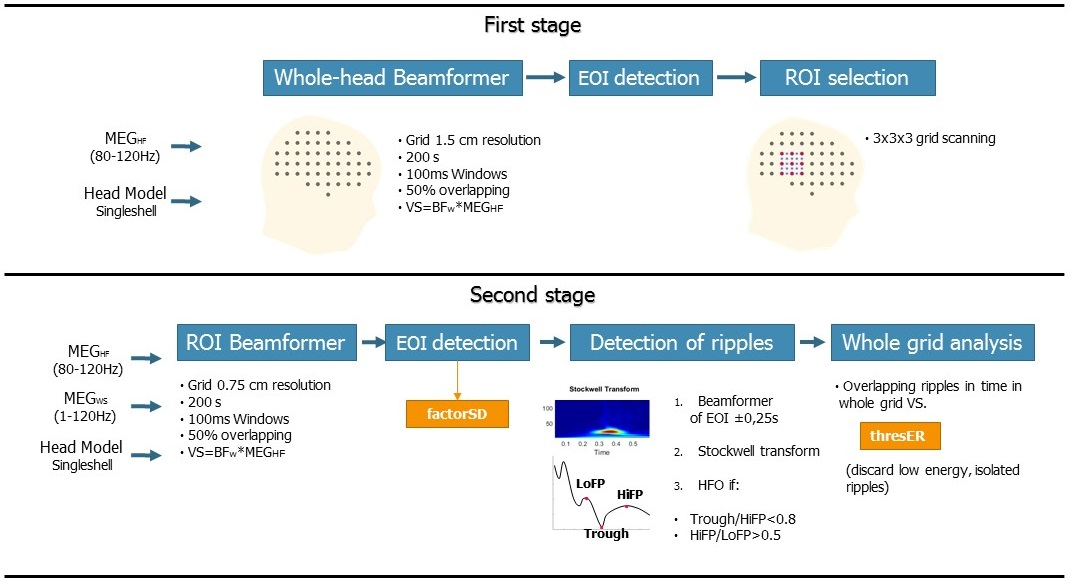
\includegraphics[width=1\textwidth]{Images/fig3-1.JPG}
\caption{Scheme of the two stages HFO detection algorithm.}
\label{fig:3-1}
\end{figure} 

\subsection{Volume conduction model}

The patient’s index points and head shape were digitized with a 3Space Fasttrack (Polhemus, Vermont, USA) prior to each measurement. The nasion, an anatomical landmark, and the left and right ear canal points served as index points and were used to define a right-handed coordinate system, called headframe coordinate system: the x-axis points to the front, the y-axis to the left, and the z-axis to the top of the head. 

The scalp and brain meshes for each subject were obtained by aligning and warping the default anatomy provided by the Montreal Neurological Institute with the Brainstorm software \citep{Tadel2011}. The volume conduction model was obtained with the single shell algorithm provided by Fieldtrip in which a realistic single shell model based on lead field expansion is computed \citep{Nolte2003}.  

\subsection{MEG automatic detection of ripples}

The proposed algorithm was divided into two main steps: 

\begin{itemize}
\item In the first step, beamforming was applied to the whole head within a coarse grid of MEG-VS to delimitate the region of interest. As beamformer computation time increases with higher resolution, this step allowed to delimitate the area of analysis in an efficient way.
\item In the second step, a second beamformer in the region of interest was computed and a finer MEG-VS grid was obtained. The automatic detection of ripples was performed with a modified version of the algorithm developed by \citep{Burnos2014}. This algorithm uses the Stockwell Transform \citep{Stockwell1996} which provides an excellent time-frequency decomposition and reduces the computational run time.  
\end{itemize}

In order to assess the performance of the proposed procedure, ripples detected in simultaneous iEEG signals were used as the gold standard. To facilitate the understanding of the whole procedure, a scheme is shown in Figure \ref{fig:3-1} and detailed explanation is provided in the next subsections.

\subsubsection*{First Stage: whole-head Beamformer and detection of the region of interest (ROI)} \label{sec:firstStage}

\begin{enumerate}[(a)]
\item \textit{Whole-head Beamformer:} The first stage was performed to define the area where the epileptic high-frequency activity was taking place. To obtain this area, a Linearly Constrained Minimum Variance Beamformer (LCMV-Beamformer) \citep{vanVeen1997} was computed to obtain the weights of the spatial filtering using an evenly spaced (1.5 cm) grid of VS including the whole brain volume of each subject. Beamformer weights ($BF_w$) were computed from $MEG_{HF}$ using sliding windows of 100ms with a 50\% overlapping. For each time segment, Virtual sensors ($VS_{HF}$) were obtained as the product of the MEGHF signals with the filter weights projecting the time-series along a unique dipole direction corresponding to the maximum variance, following the equation \ref{eq:3-1}:

\begin{equation} \label{eq:3-1}
\begin{array}{c} VS_{HF} \\ n \times s \end{array} = \begin{array}{c} BF_{w} \\ n \times m \end{array} \cdot \begin{array}{c} MEG_{HF} \\ m \times s \end{array}
\end{equation}

where \textit{n} is the number of $VS_{HF}$, \textit{m} is the number of MEG channels and \textit{s} is the length of the signal. The noise covariance was computed with the first 10 seconds of the unfiltered data \citep{vanKlink2015}. Finally, MEG-VS signals were reconstructed averaging the overlapped and successive time segments.

\item \textit{Detection of events of interest:} For each computed VSHF, events of interest (EOIs) were detected using an adapted version of the first phase of the algorithm developed in \citep{Burnos2014} for iEEG signals. For each VSHF:

\begin{enumerate}[(1)]
\item The envelope of the band-pass signal was computed with the Hilbert transform
\item The mean and the standard deviation (SD) of the envelope was computed to set a threshold equal to $ mean + 3 \cdot SD$ . 
\item An event was detected when the envelope exceeded the threshold. The duration of the event was defined as the interval between the upward and downward crossings through half the detection threshold, that was $ 0.5 \cdot (mean + 3 \cdot SD) $. 
\item If the duration of the event exceeded 6 ms, the event was qualified as an EOI.
\item EOIs with an inter-event interval of less than 10 ms were merged.
\item Events not having a minimum of 4 peaks greater than $2 \cdot SD$ from the mean baseline were rejected. 
\end{enumerate}

\item \textit{ROI selection:} Using the information provided by the EOIs, where a preliminary selection of high-frequency activity was performed discarding a fair amount of noisy events, a region with greater epileptogenic high-frequency activity could be delimitated. To do so, the number of EOIs appearing in each VSHF was computed, and all possible $3 \times 3 \times 3$ subgrids were considered and the one showing the highest number of EOIs was selected as the ROI.

\end{enumerate}

\begin{figure}[h]
\centering
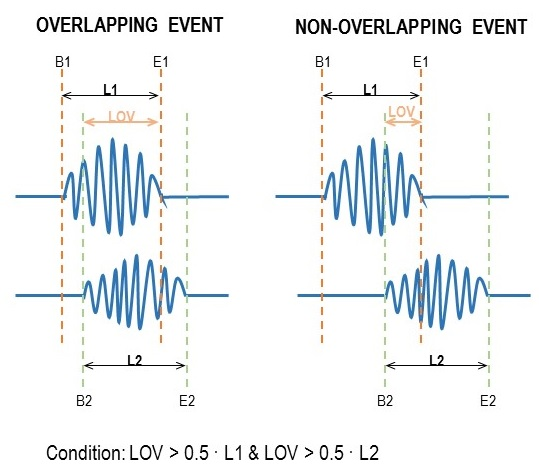
\includegraphics[width=0.6\textwidth]{Images/fig3-2.jpg}
\caption{Schematic example of the overlapping conditions. If two events had common samples and if the length of the common samples, LOV, was higher to the half of the length of the first event L1 and the second event L2, then the both events were considered as overlapping events.}
\label{fig:3-2}
\end{figure} 

\begin{figure}[h]
\centering
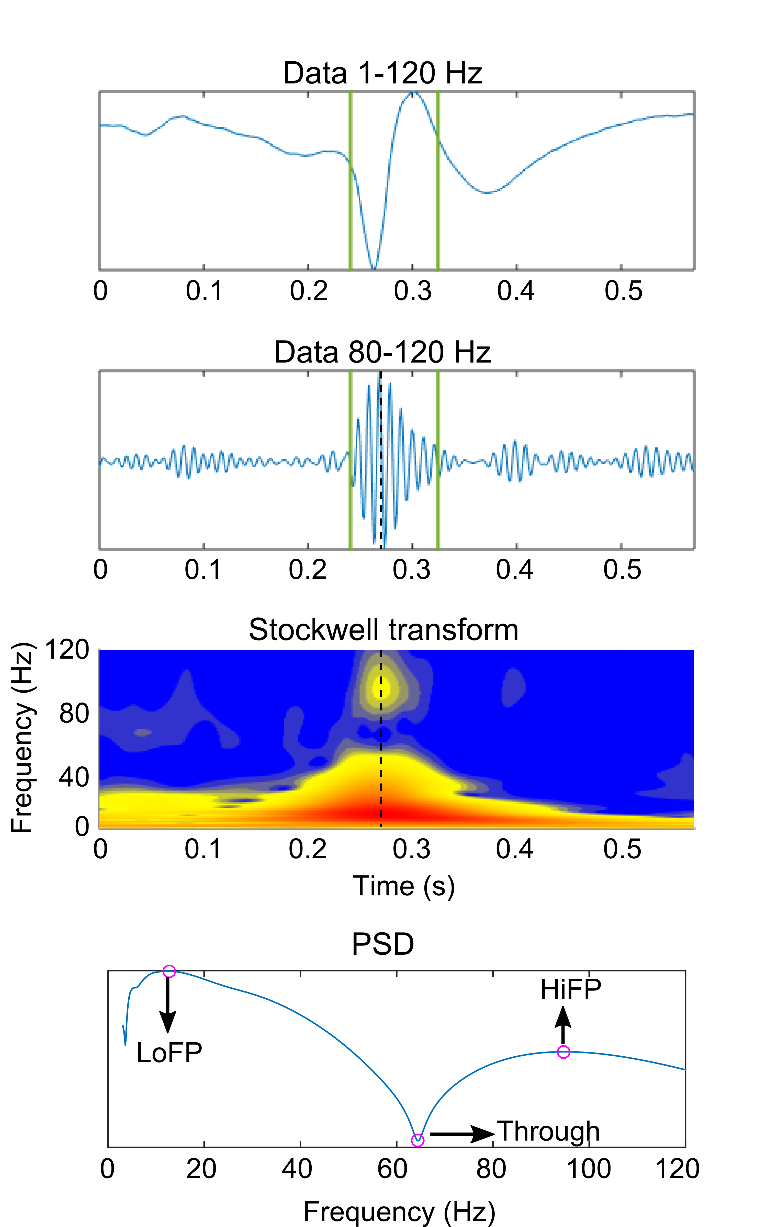
\includegraphics[width=0.4\textwidth]{Images/fig3-3.jpg}
\caption{Example of a ripple with a clear and distinguishable peak in high frequency and the selection of HiFP, Trough, LoFP in the PSD estimation at the maximum point of the envelope.}
\label{fig:3-3}
\end{figure} 

\subsubsection*{Second stage: Detection of ripples inside the ROI.}

\begin{enumerate}[(a)]
\item \textit{Beamforming inside the ROI:} A new and finer grid (0.75 cm between $VS_{HF}$) was computed inside the selected cubic ROI, creating a volume of $5 \times 5 \times 5$ points where new beamformer weights were calculated and time-series signals were obtained for each VSHF using the same procedure applied in the whole-head approach. 

\item \textit{Detection of EOIs:} EOI detection was performed for VSHF using the same algorithm explained in section \ref{sec:firstStage}. However, visual analysis of the selected segments revealed that the detection threshold of the algorithm was very restrictive and some of the events detected in iEEG that were observable in $VS_{HF}$ were not being selected as EOIs due to a lower SNR, and therefore, failed to detect a considerable number of visible events in MEG-VS. Consequently, to perform the selection of EOIs and the subsequent detection of ripples, several thresholds $ mean \pm factor_{SD} \cdot SD$ were evaluated by varying the \textit{factorSD} from 1.5 to 3 in steps of 0.25.

\item \textit{Recognition of ripples among EOIs:} The recognition of ripples among the selected EOIs was performed using a similar algorithm to the second step explained in \citep{Burnos2014}, which discards EOIs elicited by other activity than oscillatory \citep{Jacobs2012,Otsubo2008,Muthukumaraswamy2013}. The assumption taken for this step was to define a HFO as a short-lived event with an isolated spectral peak at a distinct frequency \citep{Crepon2010,Cho2012}. Beamformer was computed from $MEG_{WS}$ for each detected $ EOI \pm 0.25s $ and $VS_{WS}$ was obtained as the product of the $MEG_{WS}$ with the filter weights projecting the time-series along a unique dipole direction corresponding to the maximum variance as explained in subsection \ref{sec:firstStage}. The time-frequency response of the $VS_{WS}$ was performed using the Stockwell Transform. An event was considered a ripple if its frequency response presented a clear distinguishable peak above 80Hz. To measure this, the following steps were computed: 
  \begin{enumerate}[(1)]
  	\item The instantaneous power spectrum density (PSD) was obtained for the maximum point of the envelope (obtained by means of the Hilbert transform). An example of the computed time-frequency response and the corresponding PSD is observed in Figure \ref{fig:3-3}. 
    \item From the PSD, three parameters were computed (see Figure \ref{fig:3-3}):
    \begin{enumerate}[(i)]
    \item The high-frequency peak ($HiFP$) was selected as the spectral peak of a possible HFO. The minimum frequency of this peak is 80Hz and the maximum is 120Hz. 
    \item The $trough$ was defined as the minimum point in the range between 40Hz and $HiFP$.
    \item The low frequency peak ($LoFP$) was defined as the closest local maximum below the $trough$. 
    \end{enumerate}
\item The EOI under analysis was selected as a ripple if the following conditions were fulfilled:
    \begin{equation}
    \frac{Power(Trough)}{Power(HiFP)} < 0.8
    \end{equation}
    \begin{equation}
    \frac{Power(HiFP)}{Power(LoFP)} > 0.5
    \end{equation}
  \end{enumerate}

\item \textit{Whole grid analysis:} An additional feature was taken into account to discard ripples that appeared in just a few VS and isolated from their adjacent channels. All the detected ripples occurring at the same time segment (with a minimum of 50\% of overlapping) were assigned to the same specific ripple event. The overlapping conditions are shown in Figure \ref{fig:3-2}. The relative power of the ripple in one virtual sensor $RP(VS_i)$ was computed as follows:

\begin{equation}
RP(VS_i)=\frac{P_{event}(VS_i)-P_{200s}(VS_i)}{P_{200s}(VS_i)}
\end{equation}

where $P_{event}$ is the power in the 80-120Hz band of the ripple event in the $i^{th}$ VS and $P_{200s}$ is the power of the whole 200s signal in the same frequency band in the $i^{th}$ VS. 

The energy of an event (Er) was then computed as the sum of the maximum relative power of each VS belonging to the ripple with respect to the sum of the relative power of all the VS in that same event:

\begin{equation}
E_r=100 \cdot \frac{\sum_{n=1}^{nVS} RP(VS_n)}{\sum_{k=1}^125 RP(VS_k)}
\end{equation}

where nVS is the number of VS with a detected ripple. Once the $E_r$ was calculated, the detected ripple was discarded if its value was not high enough. The energy threshold $thres_{Er}$ was defined with the purpose of discarding isolated events or with low energy and, thereby, obtaining a better performance of the algorithm. Several values for $thres_{Er}$ were considered from 0\% to 100\% in steps of 1\%.  
\end{enumerate}

\subsection{Threshold selection: Precision/recall curves.}
The evaluation of the performance of the current algorithm was done using iEEG signals as gold standard. Ripples iEEG were automatically detected with the time-frequency analysis algorithm described in \citep{Burnos2014}. For each pair of values considered in both thresholds ($factor_{SD}$ and $thres_{Er}$) and for each automatically detected ripple in iEEG and MEG-VS, a co-occurring event was defined if these aforementioned ripples overlapped in time (see Figure \ref{fig:3-2}). Each ripple event in iEEG was considered independently for each channel. In MEG-VS, all the virtual sensors containing an overlapped event (Figure \ref{fig:3-2}) were considered as one individual event. This co-occurring ripple was considered a true positive (TP). A false positive (FP) was defined as a detected ripple in MEG-VS that was not detected in iEEG. Finally, a false negative (FN) was defined as a detected ripple in iEEG but not visible in MEG-VS. The recall (R), precision (P) and F1 score (F1) were computed as:

\begin{equation}
R = 100 \cdot \frac{TP}{TP+FN} 
\end{equation}
\begin{equation}
P = 100 \cdot \frac{TP}{TP+FP}
\end{equation}
\begin{equation}
F1 = 2 \cdot \frac{P \cdot R}{P+R}
\end{equation}

The F1 score measures the test accuracy, and can be interpreted as a weighted average of the precision and the recall. The influence of both thresholds on the discrimination of ripples from noise was evaluated by observing increases of recall or precision. To select the optimum threshold values, a leave-one-out procedure was used. The values of energy and SD threshold were computed as a function nine times, each one leaving one of the subjects out. For each of the curves, the Er and SD values that produced the higher F1 score were selected. The values selected for the classifier, $factor_{SD}$ and $thres_{Er}$ were selected using the median values for each one of the leave-one-out functions. 

\subsection{Detection and localization of ripples inside and outside the ROI} 

As mentioned before, the ROI was selected as the area with higher number of EOIs, and where the VS belonging to the ROI were expected to be more active. In order to show this hypothesis, once the automatic selection was performed and the remaining noisy events were discarded, the comparison between the number of detected ripples inside and outside the ROI was performed. For each patient, the contralateral hemisphere was selected as the area outside the ROI and the same automatic procedure to detect ripples was applied. Results were compared between the two regions.

\section{Results}

\subsection{Detection of the region of interest}

To evaluate the selected ROIs resulting from the first stage in the volume reconstruction model, the coordinates of the central virtual sensor were normalized into MNI space using brainstorm software (Figure \ref{fig:3-4}) and the gyrus and lobes were obtained for this position in the normalized atlas (Table \ref{tbl:3-2}). The central VS of the 9 subjects matched the lobe where seizures had been generated (Table \ref{tb:3-1}). 

\subsection{Threshold selection inside the ROI}

To select the values of $factor_{SD}$ and $thres_{Er}$ as the trade-off between precision and recall, the detection in iEEG and MEG-VS was compared when varying these two parameters, selecting the values that produced higher F1 score, which is, maximizing both precision and recall.  To obtain these values, a leave-one-out cross validation approach was used, in which each subject was left out and the selected values were calculated with the rest. The results of the selected values for $factor_{SD}$ and $thres_{Er}$ are shown in Table \ref{tbl:3-3}. The obtained median values were used as the final selected values: 2.25 for $factor_{SD}$ and 17.75\% for $thres_{Er}$. The averaged precision/recall and F1 score curves for all the subjects are shown in Figure \ref{fig:3-5}. A decrease of $factor_{SD}$ allowed to detect higher number of ripples increasing recall but with the risk of introducing false positive events (decreasing precision) with less energy that would appear simultaneously in a lower number of virtual sensors. This is why a similar effect was found with $thres_{Er}$: higher precision but lower recall with higher values.


\begin{figure}[h]
\centering
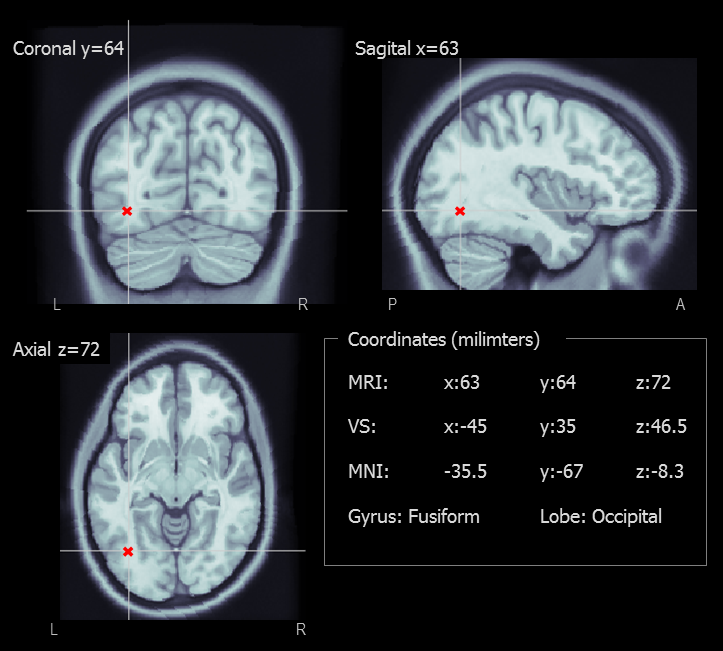
\includegraphics[width=0.65\textwidth]{Images/fig3-4.png}
\caption{Example of localization of the middle virtual sensor (in red) in the warped anatomy and the posterior MNI transformation.}
\label{fig:3-4}
\end{figure}


\subsection{Automatic detection}

The automatic detection was applied to the 9 subjects using the selected threshold values. The values of recall and precision were $68.9 \pm 0.8$ and $79.2 \pm 1.5$, respectively ($mean \pm SD$ of all subjects). The resulting F1 score was $73.7 \pm 0.6$ (TP: $25.2 \pm 10.0$; FN: $11.4 \pm 4.7$; FP: $6.6 \pm 2.5$). The average number of detected events was $31.8 \pm 12.5$, which produced a rate of ripples per minute of $9.5 \pm 3.7$, similar to the value of $6.7 \pm 4.8$ obtained by visual inspection in \citep{vanKlink2015} with MEG. The number of detected ripples in iEEG was $36.7 \pm 14.7$, producing a rate of $11.0 \pm 4.4$ ripples per minute. The detector was evaluated to ensure better-than-chance performance  \citep{Andrzejak2009} using the Poisson random probability distribution proposed in \citep{Snyder2008}. Precision, Recall and F1 score were significantly lower (p-value$<0.0001$) for the random distribution. 

Figure \ref{fig:3-6} shows, as an example, MEG-VS time-domain signals for Patient 1 after applying the beamforming algorithm. The same time segments of the iEEG channel with higher ripple rate and the 9 closest scalp-MEG channels are also shown. Ripples that are unrecognizable in scalp-MEG are observed in MEG-VS, and occur simultaneously in iEEG signals. Furthermore, the different possible situations (TP, FP, FN) of automatic detection of ripples in MEG and iEEG are shown. Table \ref{tbl:3-2} summarizes the performance of the automatic algorithm for each patient along with the global performance using the aforementioned thresholds. 


\begin{table}[!h]
\setlength{\tabcolsep}{2pt}
\centering
\caption{Brodmann Areas and lobes of the ROI and detection of ripples in MEG-VS compared to iEEG (R: right, L: left)}
\label{tbl:3-2}
\small
\vspace{3mm}
\hspace*{-0.2cm}
\begin{tabular}{llrrrrrrrr}
Patient & Gyrus/Lobe & \begin{tabular}[c]{@{}r@{}} Ripples \\ MEG-VS\end{tabular} & \begin{tabular}[c]{@{}r@{}} Ripples \\ iEEG\end{tabular} & TP & FN & FP & Recall & Precision & F1score \\ \hline 
 &         &       &      &   &    &  &       &   &     \\
1    & Fusiform/Occipital (L) & 44                        & 51                      & 35            & 16            & 9             & 68.6            & 79.5               & 73.7             \\
2    & Middle Temporal/Temporal (R)   & 48                        & 55                      & 38            & 17            & 10            & 69.1            & 79.2               & 73.8             \\
3       & Fusiform/Temporal (R)           & 54                        & 63                      & 43            & 20            & 11            & 68.2            & 79.6               & 73.5             \\
4       & Middle Temporal/Temporal (R)   & 26                        & 31                      & 21            & 10            & 5             & 67.7            & 80.8               & 73.7             \\
5       & Middle Occipital/Occipital (L) & 23                        & 26                      & 18            & 8             & 5             & 69.2            & 78.3               & 73.5             \\
6     & Superior Temporal/Temporal (L) & 17                        & 19                      & 13            & 6             & 4             & 68.4            & 76.5               & 72.2             \\
7       & Sub-gyral/Temporal (R)        & 22                        & 24                      & 17            & 7             & 5             & 70.8            & 77.3               & 73.9             \\
8       & Middle Temporal/Temporal (R)  & 25                        & 29                      & 20            & 9             & 5             & 69.0            & 80.0               & 74.1             \\
9       & Sub-gyral/Temporal (R)         & 27                        & 32                      & 22            & 10            & 5             & 68.8            & 81.5               & 74.6             \\
       &         &       &      &   &    &  &       &   &     \\
Mean   &                                  & 31.8             & 36.7           & 25.2 & 11.4 & 6.56 & 68.9   & 79.2      & 73.7    \\
SD      &                                  & 12.5             & 14.7           & 10.0 & 4.7  & 2.50 & 0.8    & 1.5       & 0.6    
\end{tabular}
\end{table}


\begin{table}[]
\centering
\caption{Optimum SD and Energy for each LOO iteration}
\small
\vspace{3mm}
\label{tbl:3-3}
\begin{tabular}{rrr}
Loo Patient & Optimum SD & Optimum $E_{HFO}(\%)$ \\
\hline
			&					  &									 \\
1           & 2.25                & 17.75                            \\
2           & 2.25                & 21.21                            \\
3           & 1.75                & 13.31                            \\
4           & 2.25                & 20.21                            \\
5           & 2.0                 & 14.79                            \\
6           & 2.25                & 17.75                            \\
7           & 2.25                & 17.75                            \\
8           & 2.25                & 17.75                            \\
9           & 2.25                & 20.21                            \\
			&					  &									 \\
Median      & 2.25                & 17.75                           
\end{tabular}
\end{table}


Note that the automated detection used for iEEG signals was based in the automatic algorithm developed in \citep{Burnos2014}, where the thresholds were trained heuristically to optimize sensitivity/specificity only in a single patient. In the current work, visual inspection of iEEG revealed that some of the events that fulfilled the Stockwell conditions were discarded in the first stage because they did not reach the threshold of $mean+3 \cdot SD$. In addition, the same authors concluded that these three times of SD could be too restrictive and high. Table \ref{tbl:3-5} shows changes in precision, recall, and F1 score values produced when the iEEG threshold was lowered to 2.5 and 2 times of SD. For this step, MEG-VS threshold values stayed invariant. An improvement in precision and F1 score values were produced when the iEEG threshold was lowered to $2.5 \cdot SD$, and only slightly lower recall values were observed. When the threshold was further decreased to $2 \cdot SD$, precision increased a bit but recall decreased more, producing a lower F1 score. These results suggested that iEEG threshold was fixed to be too restrictive for the data presented in this study and a slight lower value would have been more appropriate.

\subsection{Detection and Localization of ripples inside and outside the ROI}

The average number of detected ripples inside the ROI was $31.8 \pm 13.2$ and this value decreased to $13.4 \pm 5.0$ when computed outside the ROI ($mean \pm SD$). The number of VSWS involving each ripple event was also computed. An average number of $18.4 \pm 4.0$ VS were involved in each ripple event inside the ROI, whereas this value was slightly lower outside the ROI which showed an average of $12.6 \pm 3.8$ VS. The differences (inside and outside the ROI) between the number of detected ripples and the average number of virtual sensors were statically significant (paired T-tests, significance set to 0.05) with probability values of 0.002 and 0.02, respectively. Table \ref{tbl:3-4} shows the number of detected ripples outside the ROI and the mean number of VS involving each ripple for each patient.

\begin{table}[]
\centering
\caption{Number of ripples, mean number of MEG-VS in each ripple for all the subjects and percentage of detected ripples inside the most active region. The evaluation outside the ROI was performed placing a grid of the same size and number of channels in the contralateral hemisphere where the ROI was placed.}
\small
\vspace{3mm}
\label{tbl:3-4}
\begin{tabular}{lrrrrrr}
                 & \multicolumn{2}{c}{No. of HFOs}  & \multicolumn{2}{c}{No. of VS/HFO (mean $\pm$ sd))} & \multicolumn{2}{c}{\% Detected ripples} \\
Patient & inside ROI & outside ROI & insideROI  & outsideROI    & insideROI  & outsideROI      \\
\hline 
		&		&		&					&					&		&		\\
1       & 44    & 21    & $14.6 \pm 10.1$	& $17.7 \pm 6.4$	& 42.5 	& 14.6	\\
2       & 48    & 15    & $18.2 \pm 8.7$	& $9.2 \pm 4.1$     & 37.0	& 16.4 	\\
3     	& 54    & 21	& $21.7 \pm 16.8$	& $12.1 \pm 7.7$    & 37.9  & 13.4 	\\
4       & 26	& 14	& $22.6 \pm 8.6$	& $15.5 \pm 8.7$ 	& 34.0 	& 9.1	\\
5       & 23	& 7		& $13.1 \pm 6.3$	& $11.4 \pm 6.5$	& 32.0 	& 24.4	\\
6		& 17	& 11	& $24.7 \pm 11.5$	& $19.0 \pm 9.6$	& 28.8  & 19.3 	\\
7       & 22 	& 8		& $14.9 \pm 6.7$ 	& $14.7 \pm 7.8$ 	& 44.7  & 22.9 	\\
8       & 25	& 13	& $16.3 \pm 7.2$	& $18.5 \pm 5.3$	& 35.9 	& 17.2 	\\
9       & 27 	& 11	& $20.3 \pm 7.9$	& $15.6 \pm 11.2$ 	& 30.6 	& 16.6	\\
		&		&		&					&					&		&		\\	
Mean    & 31.8	& 13.4	& 18.4 				& 12.6				& 35.9 	& 17.1	\\
SD      & 13.2  & 5.0   & 4.0               & 3.8               & 5.3   & 4.7                                         
\end{tabular}
\end{table}




The localization maps inside and outside the ROI for Patient 1 are shown in Figure \ref{fig:3-7}. These maps measure the number of times that a specific virtual sensor was associated to a ripple. Figure \ref{fig:3-8} shows the grid inside and outside in slices (of the z-plane) for the nine subjects. These figures suggested that specific VS appeared clustered, close to each other and involved in a high number of ripples inside the ROI, showing a more focalized localization map than outside the ROI. In order to quantify this effect, the percentage of detected ripples for the most active region inside and outside the ROI is shown in Table \ref{tbl:3-4}. To compute this score, the VS showing the highest number of ripples and its six closest neighbors were selected for each subject. The ratio of the average number of ripples detected in seven clustered VS to the number of detected ripples was then computed. As expected, the percentage of ripples involved in the most active region inside the ROI was significantly higher (p-value$<0.001$) than outside the ROI. 

\begin{figure}[h]
\centering
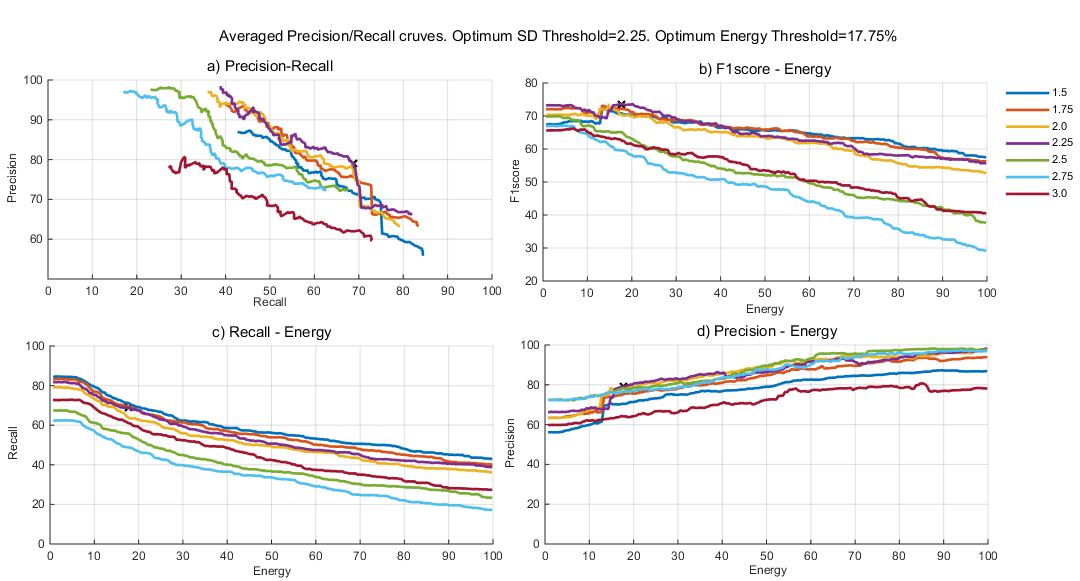
\includegraphics[width=0.65\textwidth]{Images/fig3-5.png}
\caption{Averaged performance curves. a) Precision-Recall curves for all the tested factorSD thresholds. Each value correspond to a pair of $factor_SD$ and $thres_Er$. b) F1score – Energy for all the tested thresholds. c) and d) show the recall and precision curves with respect to the energy threshold. The optimum $factor_SD$ and $thres_Er$ values were 2.25 and 17.75\% respectively.}
\label{fig:3-5}
\end{figure}

\begin{figure}[h]
\centering
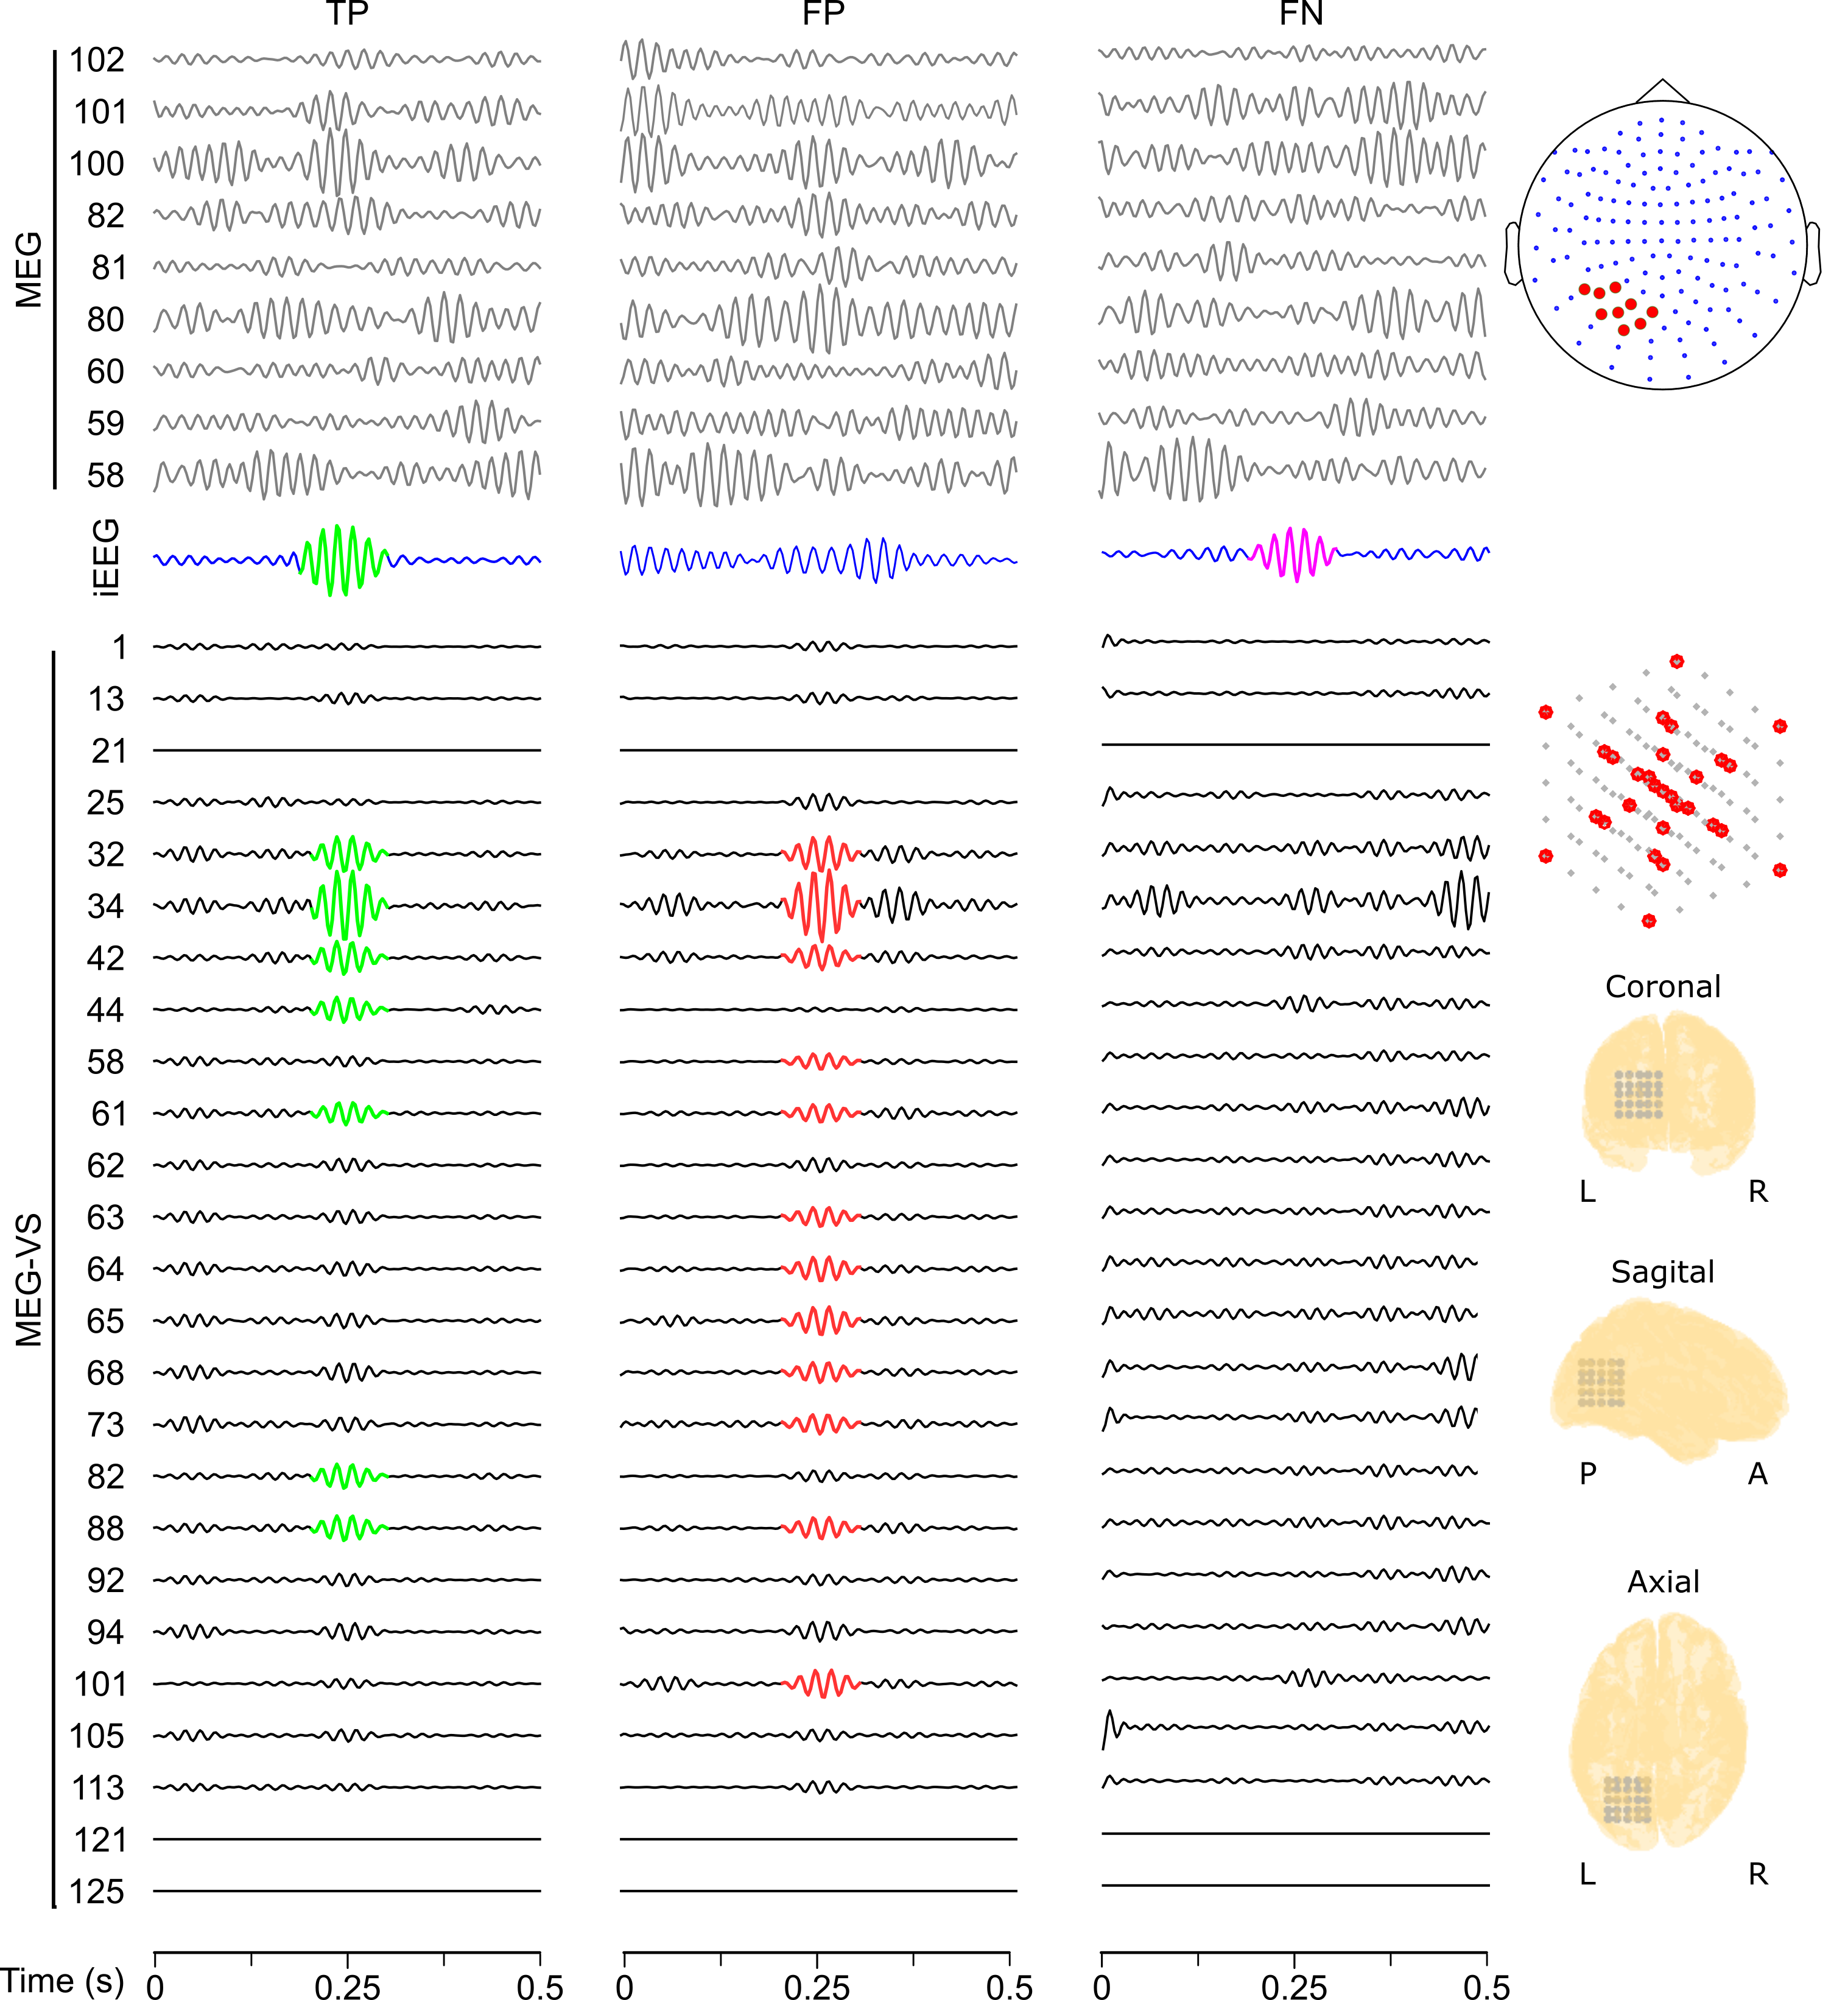
\includegraphics[width=0.7\textwidth]{Images/fig3-6.png}
\caption{Simultaneous detection of TP, FP and FN in MEG, iEEG and MEG-VS signals. MEG VS channels shown are placed on a tridimensional star-shaped configuration. MEG  channels shown belong to the nearest closest scalp area where the ROI was found. Green events correspond to a detected HFO in iEEG and MEG-VS (TP). Red events correspond to a detected HFO in MEG-VS but not visible in iEEG (FP). Pink events correspond to a detected HFO in iEEG but not visible in MEG-VS (FN). Non-labeled visible events did not meet the first conditions (EOI detection).}
\label{fig:3-6}
\end{figure}

\begin{figure}[h]
\centering
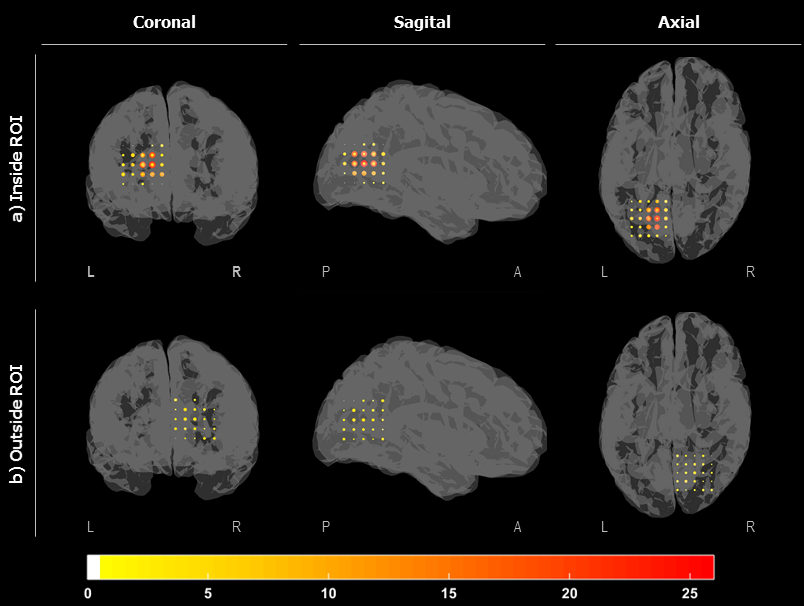
\includegraphics[width=0.85\textwidth]{Images/fig3-7.png}
\caption{Localization maps for the number of detected ripples a) inside the ROI and b) outside the ROI, on the contralateral hemisphere for Patient 1.}
\label{fig:3-7}
\end{figure}


\begin{figure}[h]
\centering
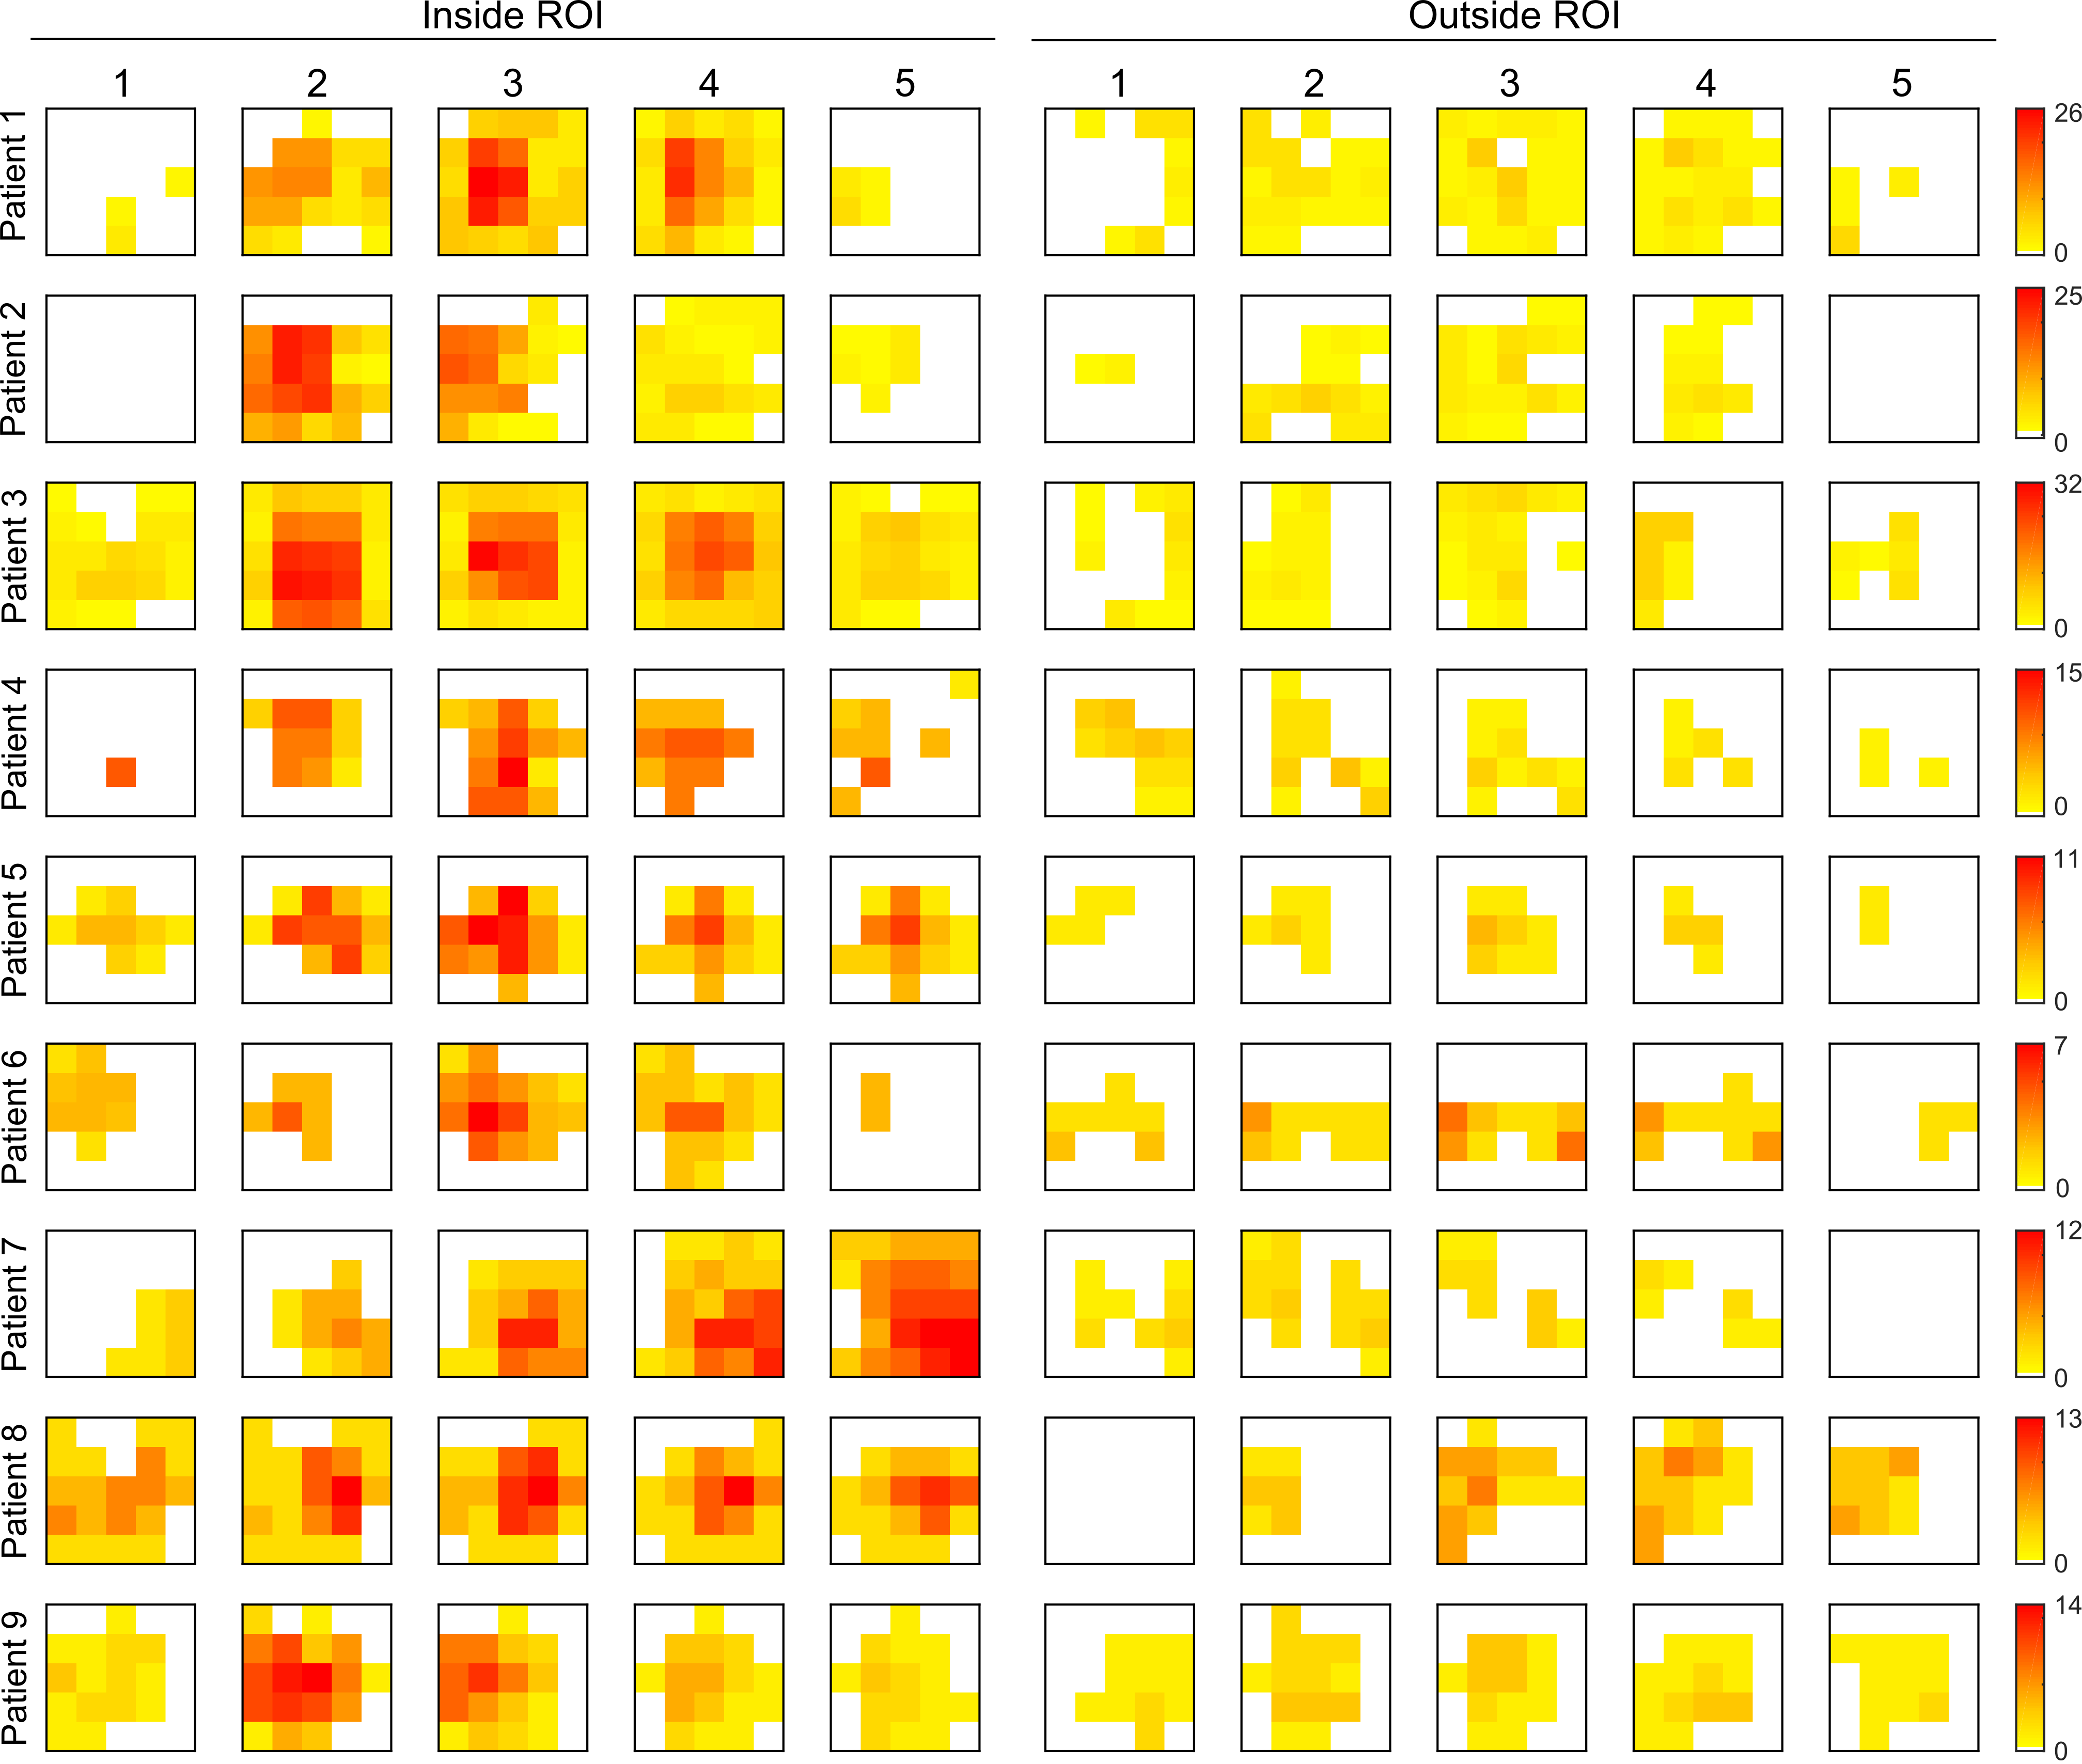
\includegraphics[width=0.95\textwidth]{Images/fig3-8.png}
\caption{Localization maps in slices of the number of detected ripples for all subjects for a) inside the ROI and b) outside the ROI. The colormap measures the number of times that a VS appeared in a ripple. }
\label{fig:3-8}
\end{figure}

\section{Discussion}

\subsection{Main contribution of the study}

There are only a few studies that identify interictal epileptic HFOs using MEG in the time domain. In \citep{vonEllenrieder2016} a semi-automatic approach was proposed to detect fast oscillations (40 Hz to 160 Hz) using MEG where the proposed algorithm was adjusted to have high sensitivity, discarding false positives by human intervention (two experts).  Visual detection of HFOs in the temporal domain is a time-consuming and highly subjective procedure. The current work represents the first study proposing an automatic approach that takes into account the time-frequency characteristics of the high-frequency events to detect ripples, while discarding other high-frequency noise events. Moreover, von Ellenrieder et al. performed the detection of ripples at the sensor level and consequently they obtained low detection rates of ripples due to the low SNR of the signals at the scalp level.  Thanks to a beamformer-based spatial filtering, a high amount of high-frequency noise reduction was achieved, allowing to discern ripples that could not be identified in scalp MEG (Figure \ref{fig:3-6}). The remaining noisy events were discarded using a two-step algorithm based on thresholds whose values were selected to maximize the correspondence with ripple events in iEEG, the current gold standard. However, beamforming algorithms can be computationally consuming, and a hybrid approach combining algorithms that detect some events at the sensor level (such as the one proposed by von Ellenrieder et al. \citep{vonEllenrieder2016}) and algorithms that are focused in the source level could provide a good compromise between computation time and detection accuracy in MEG signals.

Furthermore, the whole-head beamformer step allowed to choose the ROI without relying on epileptic spikes. The exact relationship between IEDs and HFOs remains unclear, and it is unknown whether HFOs are produced by the same generators as IEDs or not \citep{Jacobs2008}. Interictal HFOs have proven to be reliable markers of the seizure onset zone, and better than epileptic spikes \citep{Jacobs2010,Jacobs2008}. In \citep{vanKlink2015}, the authors defined a ROI based on the location of the spikes in the physical MEG sensors, but this ROI was inaccurate in two out of twelve patients. In the current study, a finer VS grid was used and fixed to the area where most high-frequency events took place, minimizing the possibilities of missing ripples occurring inside the volume of the grid. 


\subsection{Threshold selection and performance analysis}

To the best of the author’s knowledge, this is the first study that compares the simultaneous detection in time of ripples in noninvasive signals (MEG) against iEEG, the current gold standard for the detection of HFOs. Zelmann et al. \citep{Zelmann2014} had previously analyzed the spatial distribution between HFOs in iEEG and scalp EEG. In their study, the poor spatial correlation found between the two modalities was justified by the low number of channels (19 channel EEG-system), the distortion produced by the electrical conductivity of the surrounding tissues and the low SNR of the signals. The use of systems with a higher number of channels, and less influenced by the conductive properties of the skull such as MEG systems, and methods for improving the SNR of the signals, such as beamforming, provides better results in terms of localization. The automatic analysis was performed in iEEG and the values for two thresholds were selected for MEG-VS to achieve a maximum F1 score, in other words, the weighted average of precision and recall measures. Unfortunately, the exact location of iEEG in the head or the MRI of the subjects was unavailable for this study. Furthermore, the direct comparison of the recorded oscillations between these two signal acquisition methods is still uncertain. On the one hand, iEEG is an invasive technique that records electrical activity inside the head yielding a high SNR and consequently can detect events that could remain hidden in MEG signals, even after beamforming. Although there is no previous study evaluating HFOs in MEG and iEEG simultaneously in time, there are studies comparing IEDs simultaneous detection and their values of recall (or sensitivity) in MEG-VS detection with respect to iEEG which were comparable to the results of the current study, around 60-80\% \citep{Bouet2012,Huiskamp2010,Nowak2009}. While a more exhaustive comparison between the detection of IEDs and HFOs with both techniques under the same conditions should be carried out, the results on the detection should be comparable because IEDs and ripples have similar SNR values at their respective frequency bands \citep{vonEllenrieder2012}, and because signals are equally attenuated at all frequencies of interest \citep{Zelmann2014}. On the other hand, MEG can often provide additional and useful information mainly because of its whole-head coverage while iEEG recordings usually only provide a locally limited neurophysiological picture \citep{Muthukumaraswamy2013}. The number of depth electrodes for this study covered a small region of the brain. For this reason, there is still some uncertainty regarding the FP ripples because they could be either noise being incorrectly detected as HFOs or actual ripples not recorded by iEEG. 


\begin{table}[!h]
\centering
\caption{Average values of performance (Precision, Recall and F1 score) and number of Co-detected Events, Detected Events only in iEEG, and detected events only in MEG when iEEG SD threshold was lowered.  The duration of the EOI was set to $0.5 \cdot (mean+3\cdot SD)$ for the three evaluated thresholds}
\small
\vspace{3mm}
\label{tbl:3-5}
\begin{tabular}{rccc}
iEEG SD                 & 3.0 & 2.5 & 2.0 \\
\hline 
						&			   &			  &				 \\
Co-detected Events      & 25.2         & 26.2         & 26.4         \\
Detected Events in iEEG & 11.4         & 12.0         & 13.5         \\
Detected events in MEG  & 6.7          & 5.6          & 5.4          \\
Recall                  & 68.9         & 71.2         & 70.1         \\
Precision               & 79.2         & 82.4         & 83.0         \\
F1 score                & 73.7         & 76.4         & 76.0         \\
\end{tabular}
\end{table}

The automatic detection of HFOs in invasive records is still an open field of study \citep{Liu2016,Burnos2014}. For all these reasons, using the iEEG as gold standard implies the acceptance of the detection provided by this technique. Table \ref{tbl:3-5} shows that changing the SD threshold in the iEEG automatic detection produced variations in the number of co-detected events, suggesting that the threshold proposed in \citep{Burnos2014} might be fairly restrictive depending on the characteristics of the signals. The abovementioned selection of values for both thresholds considered the highest values of F1 scores, but they could be selected different depending on the purpose of the detection: The values of $factor_{SD}$ and $thres_{Er}$ could be decreased to maximize recall (higher than 80\%) and to detect the highest possible number of ripples or, conversely, they could be increased to maximize precision (around 95\%) and ensure almost totally that the detected events were equally visible in iEEG and MEG-VS. Nonetheless, more efforts should be directed to provide a reliable detection of ripples in MEG-VS by observing other characteristics of the actual signals (such as HFOs onsets or connectivity between VS) or taking into account post-surgical outcomes (which were not available in this database). 

\subsection{Evaluation of ripples inside and outside the ROI}

An automatic selection of the area that showed the highest number of EOIs was performed to circumscribe the detection of ripples to a volume of approximately $9 cm^3$. This area agreed with the affected zone targeted by clinicians (Tables \ref{tb:3-1} and \ref{tbl:3-2}). The HFO detection algorithm was applied to the same volume in the contralateral hemisphere with the purpose of comparing the number of ripples and the pattern drawn by VSWS involved (Figures \ref{fig:3-6} and \ref{fig:3-7}). In general, a group of VS that were detected simultaneously in different ripples produced a focalized map inside the ROI. Although this information was still insufficient to provide a reliable localization of the area generating pathological HFOs because of the lack of precise clinical information, it could be inferred that the oscillations were mostly generated by a common focus and this provides a general idea of the area where the ripples appeared. It is important to remark that although the automatic detection algorithm use a ROI to detect ripples, these can be mapped a posteriori throughout the head, using the temporal information about the detected ripple segments.

The proposed algorithm also detected some ripples outside the ROI but the number of events was significantly lower and involved fewer VS. There is still uncertainty between the differential characteristics and mechanisms of pathological and physiological ripples \citep{Jefferys2012}. Whether all the detected events were actually physiological, pathological, or noise cannot be definitely be demonstrated, but the detected ripples outside the ROI presented lower values of energy, which is a characteristic of physiological HFOs \citep{Matsumoto2013}. Moreover, the pattern of these oscillations appeared more scattered throughout the volume, indicating that these oscillations were not generated by a common area or focus. This finding is in correspondence to the observations with animal studies indicating that the areas generating physiological HFOs appeared more extended \citep{Chrobak1996} than the areas generating pathological HFOs, that are smaller brain regions on the order of cubic millimeters \citep{Bragin2002}. The results from \citet{Zelmann2014} suggested that it is possible to measure the activity from small cortical regions at the scalp level. This could be explained by the solid angled concept introduced by \citet{Gloor1985}. These measures should be comparable with those obtained with subdural grid contacts, always taking into account that the spatial resolution of the technique should be high.

\subsection{Limitations of the study and further work}

Beamformer virtual sensors allowed the detection of high-frequency activity otherwise not observable by the physical sensors. The main purpose of this study was to automatically detect ripple events in MEG and discern them from noise by analyzing time-frequency characteristics using iEEG recordings to adjust and validate the algorithm. However, due to the lack of spatial location of intracranial electrodes, only a full-scale spatial validation of the detected ripples could be performed. 

The spatial resolution of the reconstructed virtual sensors is limited and depends on the depth, position and orientation of the sources, the SNR of the raw data, and the geometry of the head \citep{Hillebrand2002}. For all of these reasons, beamformer-based methods are not suitable for clinical application yet for the localization of the epileptic focus through ripples and the replacement of invasive techniques. However, the automatic detection in non-invasive techniques could be useful to guide the implantation of intracranial electrodes of subdural grids as it has been demonstrated that HFOs delimitate the affected area better than IEDs \citep{Jacobs2008}.

More efforts should be put to increase the SNR of the signals, and in this sense independent component analysis has proven to be effective improving the spatial localization of beamformer spatial filters \citep{Fatima2013}. Ultra-low-noise EEG/MEG techniques \citep{Fedele2015} are promising in the noninvasive detection of HFOs. Moreover, using the actual MRI of each subject to compute the head model would produce better results in the localization of the epileptic sources. A complete analysis comparing MEG with intracranial recordings should also include the position of implantation of the subdural electrodes. 
Furthermore, using MEG systems with more channels and higher frequency rates would provide a better spatial and temporal resolution. Several studies have found that fast ripples have shown to be more correlated with the seizure onset zone and presumably highly epileptogenic \citep{vanKlink2014,Zijlmans2012,Haegelen2013,Jacobs2008} than ripples. Due to the sampling rate limitation, this study only analyzed ripples up to 120Hz. However, the automatic detection algorithm does not depend on the sampling rate and can be used to detect HFOs of higher frequency content acquired at higher rates. This would allow evaluating the differences in localization of ripples and fast ripples and their relationship with the seizure onset zone. Furthermore, fast ripples would likely be downsampled to appear at lower harmonics, being able to detect them, but not to classify them between ripples or fast-ripples. Moreover, the study of ripples by non-invasive methods can also help to lateralize the epileptic focus in secondary bilateral synchrony \citep{Pizzo2016}, delimitate the seizure onset zone in patients where fast ripples are not visible \citep{vanKlink2014}, and in general, provide a better delimitation of the affected area than IEDs \citep{Jacobs2008}. Moreover, the detection of this area with non-invasive techniques can provide relevant information to guide the implantation of intracranial electrodes and for surgical treatment \citep{vonEllenrieder2016}. It is important to highlight that computation time increases with frequency and spatial resolution. These algorithms should be implemented efficiently minimizing the computation time to be suitable for clinical analysis. 

Finally, improving the spatial and temporal resolution would also allow to detect HFOs and determine the SOZ in the whole head using automated methods and clustering analysis, computing different features such as density, connectivity, peak frequency, power, amplitude \citep{Modur2015},  or spectral entropy \citep{Liu2016}. The automatic detection algorithm presented in this study would also be useful to extend these studies, which are currently limited for iEEG, would exploit the advantage of the whole head coverage of MEG allowing the assessment of the neural mechanisms of epilepsy as well as reducing invasiveness in clinical patients. The comparison between the areas of the brain generating HFOs and IEDs in epilepsy and its relationship would also be an interesting field of study. Moreover, a careful analysis of the whole brain volume could allow to understand the areas involved in the HFO generation, the propagation of this activity and how they are related with the epileptogenic networks. 


\section{Conclusion}

High-frequency oscillations are promising biomarkers for epilepsy. Several studies detect them automatically in intracranial recordings, but there are few studies evaluating these oscillations in noninvasive signals. To the authors’ knowledge, this is the first study dealing with full automatic detection of ripples in MEG in the time domain taking into account the time-frequency characteristics of the events through the whole signal spectrum. Moreover, these ripples corresponded to the clinically expected epileptogenic area. The detection was compared with intracranial EEG recordings, demonstrating that the identification of ripples in MEG is feasible. The noninvasive study of HFOs is an interesting field of study that would allow to evaluate HFO mechanisms in larger groups of epileptic patients and also in healthy subjects to discern the differences between pathologic and physiologic fast oscillations. 


\section{Acknowledgments}

CIBER-BBN is an initiative of the Instituto de Salud Carlos III, Spain. This work has been partially supported by the Ministry of Economy and Competitiveness, Spain, under contract DPI2014-59049-R and the Ministry of Education, Culture and Sports FPU12/05631. We thank Sylvain Baillet and its group NeuroSpeed (Montreal Neurological Institute, McGill University) for the help and comments during the course of this research that greatly improved this work. 




